\documentclass{article}

% ── Packages ──────────────────────────────────────────────────────────────────
\usepackage[margin=1in]{geometry}
\usepackage{times}
\usepackage{amsmath,amssymb}
\usepackage{graphicx}
\usepackage{booktabs}
\usepackage{multirow}
\usepackage{hyperref}
\usepackage{natbib}
\usepackage{caption}
\usepackage{subcaption}
\usepackage{float}
\usepackage{microtype}
\usepackage[T1]{fontenc}
\usepackage[utf8]{inputenc}

\hypersetup{colorlinks=true, linkcolor=blue, citecolor=blue, urlcolor=blue}

\title{\textbf{Predicting Citi Bike Station Demand in New York City}\\
\large DS-GA 1003 Final Project}

\author{
  Jing Yu \quad Huijing Cong \quad Elaine Zhou \\
  New York University
}
\date{}

% ── Document ──────────────────────────────────────────────────────────────────
\begin{document}
\maketitle

% ── Abstract ──────────────────────────────────────────────────────────────────
\begin{abstract}
Bike-sharing systems like NYC Citi Bike face persistent supply imbalances caused
by uneven, time-varying demand across stations. We formulate hourly station-level
departure count prediction as a regression problem and build a full machine
learning pipeline over two years of Citi Bike trip records (January 2023 –
December 2024), covering approximately 1,700 active stations and over 43 million
station-hour observations. We compare six models — Ridge Regression, Random
Forest, XGBoost, MLP, LightGBM, and a hyperparameter-tuned LightGBM — and find
that the tuned LightGBM achieves a test RMSE of \textbf{1.501} and MAE of
\textbf{0.759} departures per hour. Analysis reveals that short-term lag
features dominate predictive performance, PM rush hour is the hardest time to
predict, and high-error stations concentrate in high-demand Midtown Manhattan.
\end{abstract}

% ── 1. Introduction ───────────────────────────────────────────────────────────
\section{Introduction}

Citi Bike is the largest bike-sharing system in New York City, with stations
spread across Manhattan, Brooklyn, Queens, and the Bronx. A core operational
challenge is that demand is spatially and temporally uneven: some stations run
out of bikes while others overflow, forcing costly manual rebalancing operations.
Accurate short-term demand forecasts can help operators anticipate these
imbalances and act proactively.

In this work, we study whether station-level bike demand can be predicted using
historical trip data combined with weather and calendar information. We
formulate the task as a regression problem: given a station and a specific hour,
predict the number of bike departures in that hour. We train and evaluate models
on two full years of data and conduct detailed analyses to understand when and
where predictions are most and least reliable.

% ── 2. Related Work ───────────────────────────────────────────────────────────
\section{Related Work}

Several prior studies have applied machine learning to bike-sharing demand
forecasting, using a range of datasets, spatial granularities, and modeling
approaches.

\citet{torres2024forecasting} directly study hourly station-level demand on
the NYC Citi Bike system — the same dataset we use — and compare Random Forest,
Gradient Boosting, and Artificial Neural Networks with calendar and weather
features. They find that all three methods achieve similar accuracy, and
recommend Random Forest for its simplicity. Our work extends this line of
research in two key ways: we include explicit lag features (demand 1, 2, and 24
hours prior), which we show account for 85\% of predictive gain, and we evaluate
LightGBM with systematic hyperparameter tuning via Optuna, which outperforms
standard Gradient Boosting.

\citet{zhou2024stgcn} also work on NYC Citi Bike and propose a deep
learning approach based on Spatio-Temporal Graph Convolutional Networks
(ST-GCN) with temporal convolutions and self-attention, explicitly modeling
spatial dependencies between stations. Their model achieves a test RMSE of 2.36
and MAE of 1.62. Our tuned LightGBM achieves RMSE = 1.501 and MAE = 0.759,
which is considerably better, suggesting that strong lag features and careful
feature engineering can outperform graph neural network approaches on this task
while being far simpler to implement and train.

\citet{cortez2023scalability} evaluate a broader set of methods —
including ARIMA, Linear Regression, Random Forest, Prophet, and XGBoost — on
three bike-sharing systems of different scales: Logroño (23 stations),
Barcelona (519 stations), and NYC Citi Bike (1,500+ stations). They find that
NYC is the hardest system to forecast, with the highest normalized error across
all methods, and that no single algorithm generalizes best across all system
sizes. Their work motivates our focus on strong gradient boosting methods for
large-scale systems, and highlights that XGBoost is competitive on the NYC
system — a result that we replicate and extend with LightGBM.

\citet{hosseinpanahi2026ml} study hourly demand forecasting on the
Chicago Divvy system using cluster-level aggregation and compare Linear
Regression, ARIMA, and Random Forest with weather features. They achieve up to
$R^2 = 0.80$ at the cluster level. While their city and spatial aggregation
differ from ours, their work supports the general value of ML-based hourly
forecasting for North American bike-sharing systems and confirms that weather
variables provide useful signal alongside temporal features.

Taken together, prior work establishes the value of tree-based models and
weather/temporal features for hourly BSS demand forecasting, but no prior study
on this dataset has combined explicit lag features, large-scale training, and
systematic hyperparameter tuning. Our work fills this gap.

% ── 3. Data ───────────────────────────────────────────────────────────────────
\section{Data}

\subsection{Sources}

We use three data sources. The primary source is the \textbf{Citi Bike System
Data}, a public dataset of individual trip records available from the Citi Bike
S3 archive. Each record includes ride type, start and end timestamps, start and
end station IDs, station coordinates, and rider type (member or casual). We use
trip data from January 2023 through December 2024 and aggregate raw records into
hourly departure counts per station, which serve as our prediction target.

The second source is the \textbf{Open-Meteo Archive API}, which provides hourly
historical weather observations from the Central Park station. We use
temperature ($^\circ$F), precipitation (inches), snowfall (inches), and snow
depth (inches). Although a single weather station cannot capture fine-grained
local variation across the city, it captures major weather events that affect
citywide ridership.

The third source is the Python \texttt{holidays} package, which provides a
binary indicator for New York State federal holidays. Biking patterns on
holidays differ noticeably from regular weekdays.

\subsection{Preprocessing and Feature Engineering}

We aggregate raw trip records into a station $\times$ hour demand grid. Hours
with zero departures are explicitly filled with zeros so that lag features can
be computed correctly. The full grid covers 1,704 active stations and 17,520
hourly time slots, producing approximately 43.6 million station-hour rows.

For each row, we construct the following features:

\begin{itemize}
  \item \textbf{Time features:} hour of day (0--23), day of week (0--6),
        month (1--12), binary weekend indicator, binary holiday indicator.
  \item \textbf{Station features:} latitude and longitude.
  \item \textbf{Weather features:} temperature, precipitation, snowfall,
        snow depth (all from the Central Park station).
  \item \textbf{Lag features:} departures at the same station 1, 2, and 24
        hours prior. These capture short-term autocorrelation and the
        same-hour-yesterday pattern.
\end{itemize}

The first 24 hours of each station's history are dropped because lag values are
unavailable, leaving approximately 43.6 million usable rows.

\subsection{Train / Validation / Test Split}

To avoid data leakage, we use a time-based split:

\begin{center}
\begin{tabular}{lll}
\toprule
Split & Period & Approx.\ rows \\
\midrule
Train & Jan 2023 -- Sep 2024 & 38M \\
Validation & Oct -- Nov 2024 & 3M \\
Test & Dec 2024 & 1.85M \\
\bottomrule
\end{tabular}
\end{center}

This setup mirrors real-world deployment, where a model trained on historical
data must generalize to future time periods.

% ── 4. Methods ────────────────────────────────────────────────────────────────
\section{Methods}

We train and compare six models with increasing complexity.

\textbf{Ridge Regression} serves as our linear baseline. It models the target
as a weighted sum of features with L2 regularization and provides a lower bound
on nonlinear methods.

\textbf{Random Forest} \citep{ke2017lightgbm} is a nonlinear ensemble of
decision trees that captures feature interactions without requiring feature
scaling. Due to memory constraints, it is trained on a 5M-row random subsample
of the training set.

\textbf{XGBoost} \citep{chen2016xgboost} is a gradient boosting framework that
builds trees sequentially to minimize residuals. It uses early stopping on the
validation set and is trained on the full 38M-row training set.

\textbf{MLP (Multi-Layer Perceptron)} is a two-hidden-layer neural network
trained on the same 5M-row subsample as Random Forest, using standardized
inputs.

\textbf{LightGBM} \citep{ke2017lightgbm} is a highly efficient gradient
boosting library that uses histogram-based tree learning. It is trained on the
full 38M-row training set with early stopping.

\textbf{LightGBM (tuned)} uses the same algorithm but with hyperparameters
optimized via Optuna \citep{akiba2019optuna} Tree-structured Parzen Estimator
(TPE) search over 30 trials on a 5M-row subsample, then retrained on the full
38M-row set with the best hyperparameters. Key tuned parameters include
\texttt{num\_leaves=457}, \texttt{learning\_rate=0.0183},
\texttt{feature\_fraction=0.742}, and \texttt{reg\_lambda=9.4}.

All models are evaluated using Root Mean Squared Error (RMSE) and Mean Absolute
Error (MAE), computed on both the validation and test sets. RMSE penalizes large
errors more heavily, which is relevant when predicting demand spikes. MAE gives
the average per-hour prediction error in number of departures.

% ── 5. Results ────────────────────────────────────────────────────────────────
\section{Results}

Table~\ref{tab:results} reports RMSE and MAE for all six models on the
validation and test sets.

\begin{table}[H]
\centering
\caption{Model performance on validation (Oct--Nov 2024) and test (Dec 2024) sets.
         RF and MLP are trained on a 5M-row subsample; all others use 38M rows.}
\label{tab:results}
\begin{tabular}{lcccc}
\toprule
Model & Val RMSE & Val MAE & Test RMSE & Test MAE \\
\midrule
Ridge Regression     & 2.626 & 1.345 & 1.720 & 0.841 \\
Random Forest        & 2.288 & 1.183 & 1.566 & 0.808 \\
MLP                  & 2.249 & 1.169 & 1.564 & 0.792 \\
XGBoost              & 2.232 & 1.172 & 1.536 & 0.788 \\
LightGBM             & 2.137 & 1.129 & 1.503 & 0.769 \\
LightGBM (tuned)     & \textbf{2.098} & \textbf{1.099} & \textbf{1.501} & \textbf{0.759} \\
\bottomrule
\end{tabular}
\end{table}

The tuned LightGBM achieves the best performance on both splits. Compared to
Ridge Regression, it reduces test RMSE by 12.7\% and MAE by 9.7\%. The gap
between LightGBM and the other nonlinear models is relatively small — XGBoost
comes close (test RMSE 1.536) — but LightGBM's efficiency on the full 38M-row
training set gives it an advantage over Random Forest and MLP, which require
subsampling. Hyperparameter tuning provides only a marginal additional gain over
the default LightGBM (0.002 RMSE), suggesting the model is already well-suited
to this task out of the box.

Our test RMSE of 1.501 compares favorably against \citet{zhou2024stgcn}, who
report RMSE = 2.36 on the same system using a graph neural network, and against
simpler baselines reported in \citet{cortez2023scalability}.

% ── 6. Analysis ───────────────────────────────────────────────────────────────
\section{Analysis}

\subsection{Feature Importance}

\begin{figure}[H]
  \centering
  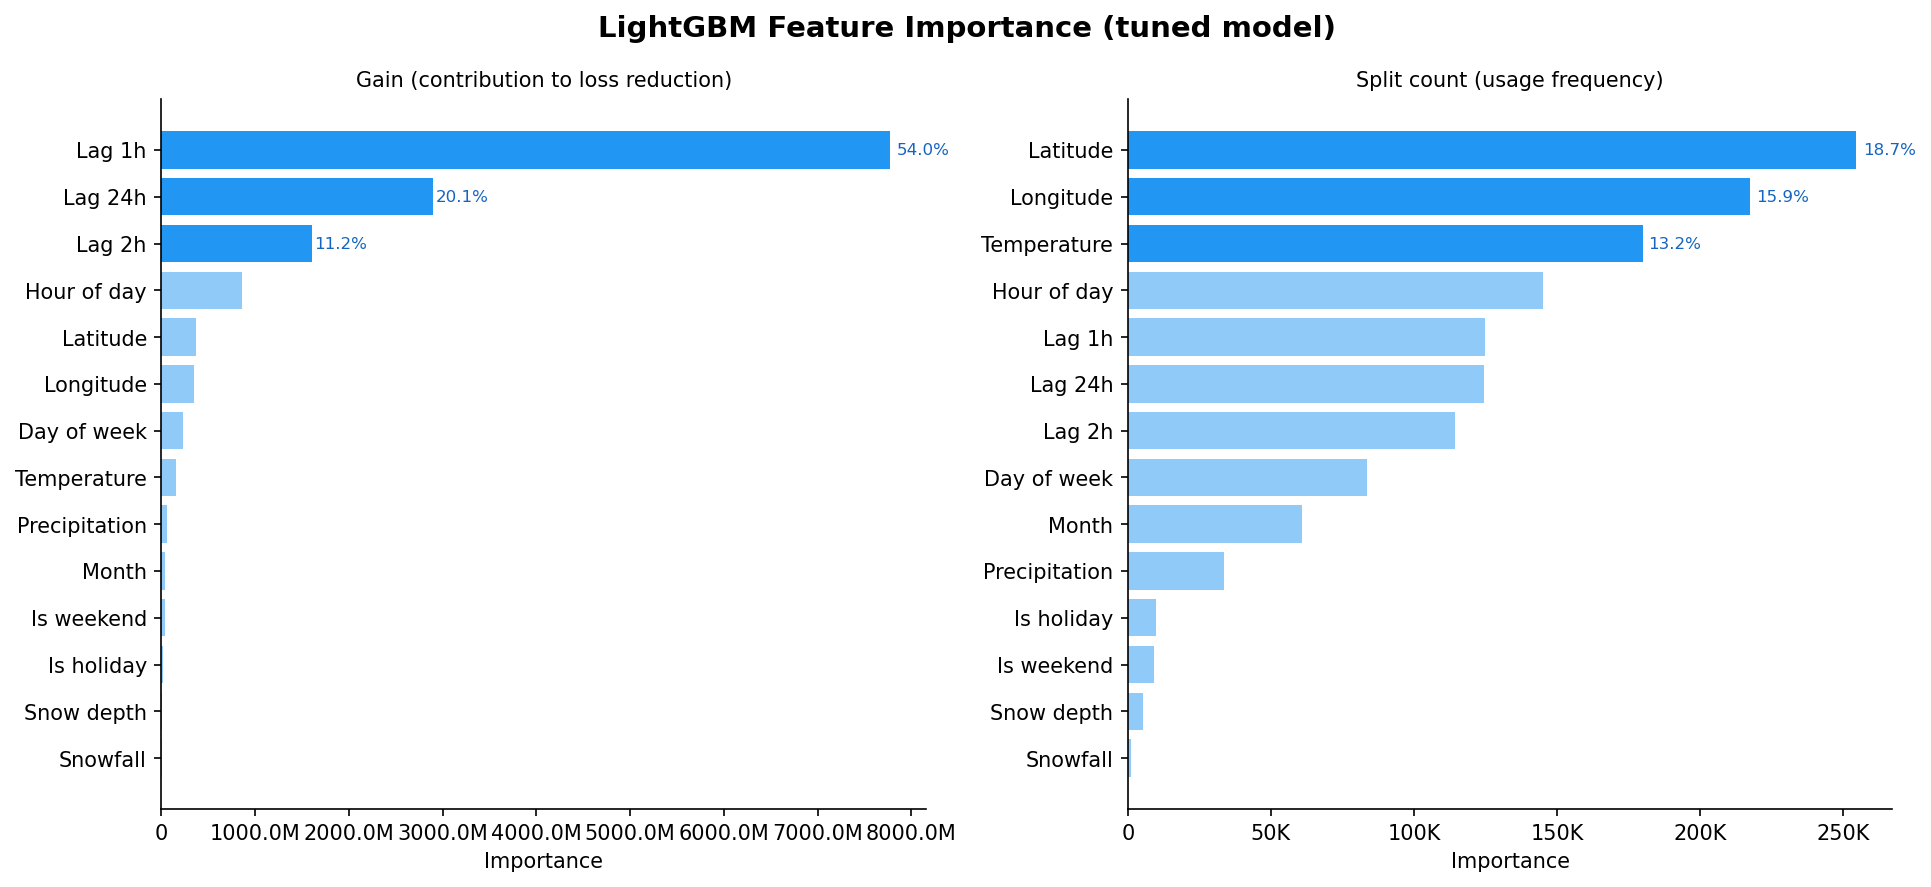
\includegraphics[width=0.75\linewidth]{../results/feature_importance.png}
  \caption{Feature importance (gain) for the tuned LightGBM model.}
  \label{fig:importance}
\end{figure}

Figure~\ref{fig:importance} shows feature importance measured by gain (total
reduction in loss attributed to each feature). The three lag features together
account for \textbf{85\%} of total gain: \texttt{lag\_1h} alone contributes
54.0\%, \texttt{lag\_24h} contributes 20.1\%, and \texttt{lag\_2h} contributes
11.2\%. This confirms that short-term autocorrelation is the dominant signal for
hourly demand prediction. The same-hour-yesterday lag (\texttt{lag\_24h})
captures daily rhythms, while \texttt{lag\_1h} and \texttt{lag\_2h} capture
short-term momentum.

Hour of day (5.9\%) and station coordinates (5.0\% combined) are the next most
informative features. Weather variables, day of week, and holidays together
account for only about 3\% of gain. While their individual contribution is
small, they are still included because they improve calibration for edge cases
(e.g., snowstorms, holidays) where patterns deviate from recent history.

\subsection{Error Distribution}

\begin{figure}[H]
  \centering
  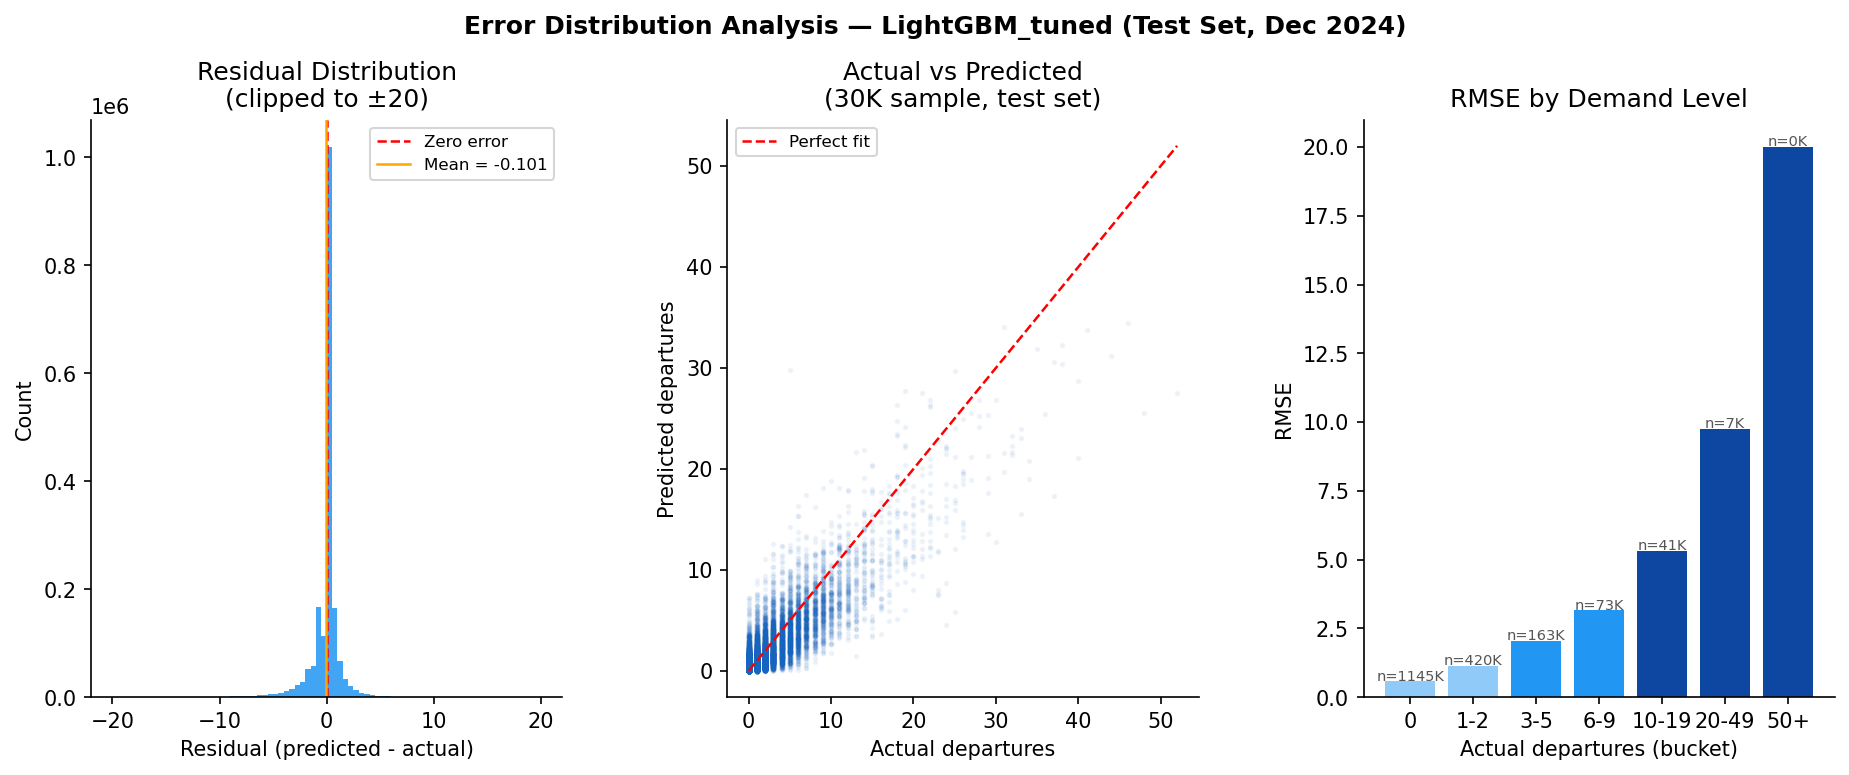
\includegraphics[width=0.75\linewidth]{../results/error_distribution.png}
  \caption{Residual distribution and RMSE by demand bucket on the test set.}
  \label{fig:error}
\end{figure}

Figure~\ref{fig:error} shows the distribution of residuals (predicted minus
actual) on the test set. The mean residual is $-0.101$, indicating a very slight
tendency to underestimate. The distribution is sharply peaked near zero, with
68.5\% of predictions above the actual value. This overestimation bias occurs
mainly because 62\% of test rows have zero departures, and the model assigns
small positive predictions to many of these quiet hours.

RMSE scales strongly with demand level: for zero-departure hours, RMSE is 0.57;
for the 79 extreme-demand hours with 50+ departures, RMSE reaches 20. This
pattern suggests that the model has learned the typical demand level well, but
struggles to capture demand spikes driven by events or unusual conditions.

\subsection{Temporal Error Analysis}

\begin{figure}[H]
  \centering
  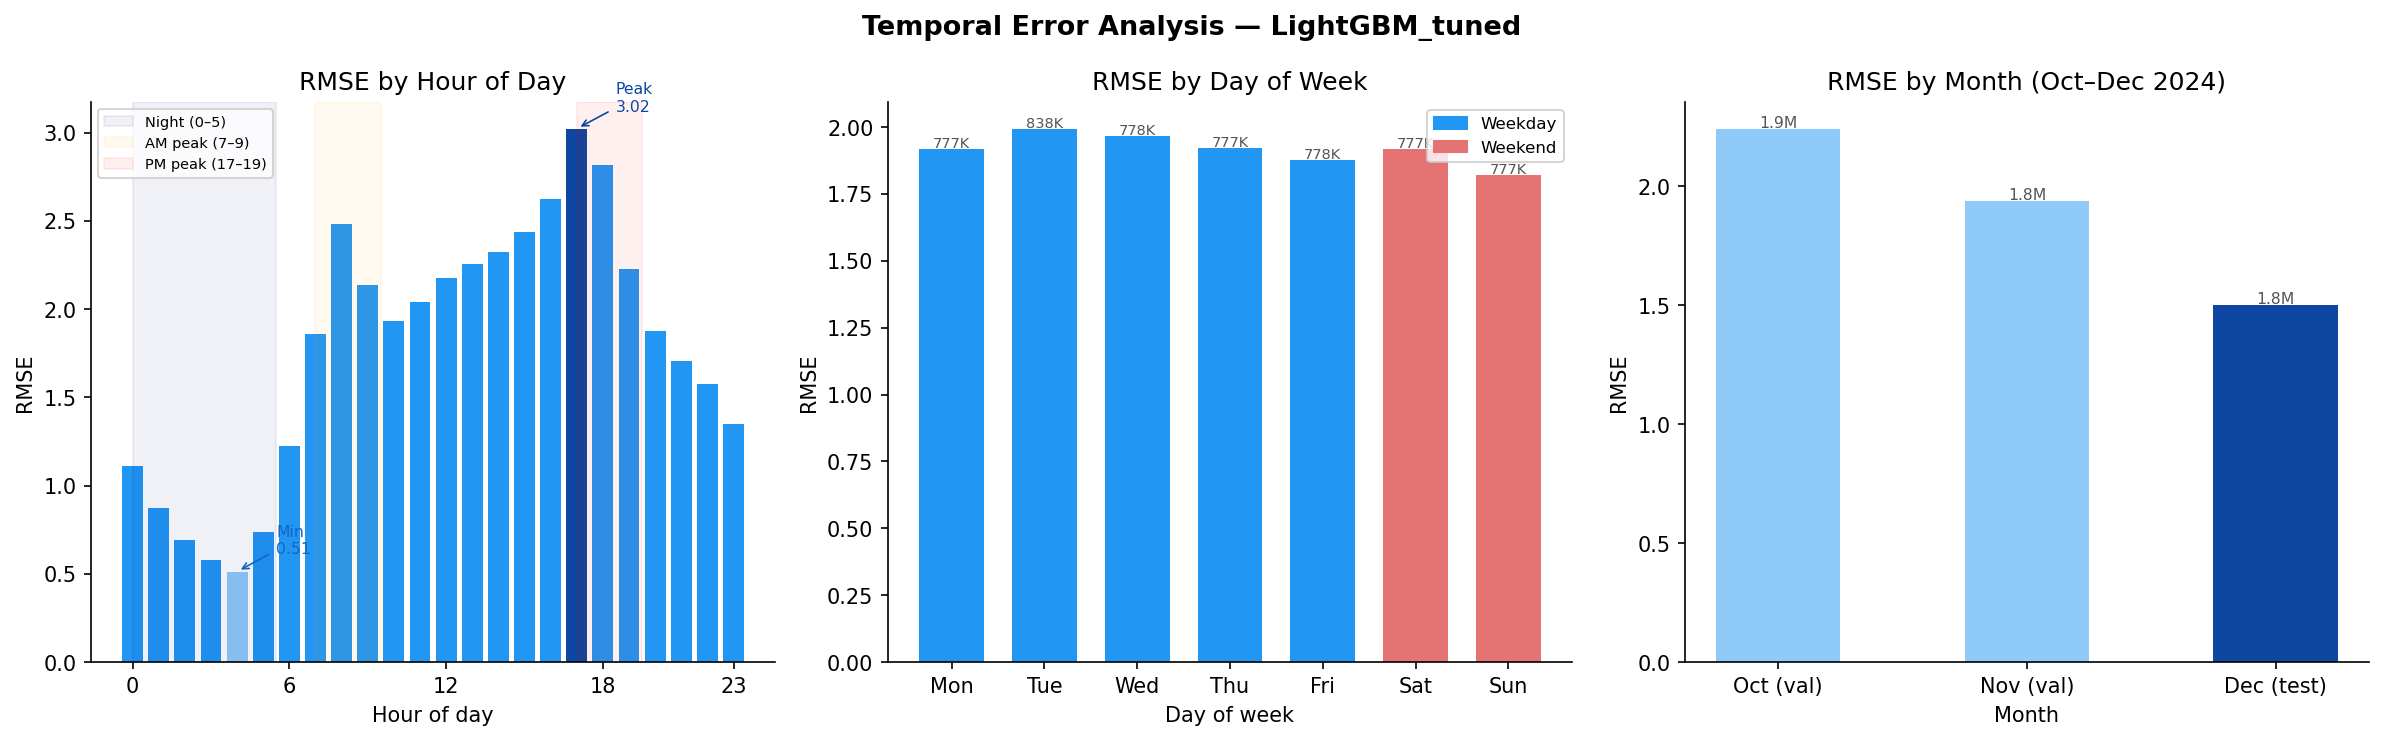
\includegraphics[width=0.95\linewidth]{../results/temporal_error.png}
  \caption{Test RMSE by hour of day, day of week, and month.}
  \label{fig:temporal}
\end{figure}

Figure~\ref{fig:temporal} shows how prediction error varies across time. The PM
rush hour (17:00) is the hardest time to predict, with RMSE = 3.02 — about six
times higher than the overnight minimum of 0.51 at 4:00 AM. The morning commute
(7:00--9:00) also shows elevated errors (RMSE 1.86--2.48). These high-demand
periods have more volatile ridership that is difficult to capture with lag
features alone.

Day of week has little effect: RMSE ranges from only 1.82 on Sunday to 1.99 on
Tuesday, a 9\% spread. Errors decrease as winter progresses: October val RMSE
is 2.24, November is 1.94, and December test RMSE is 1.50. This is partly
because colder weather reduces overall demand, leading to fewer extreme spikes.

\subsection{Per-Station Error Analysis}

\begin{figure}[H]
  \centering
  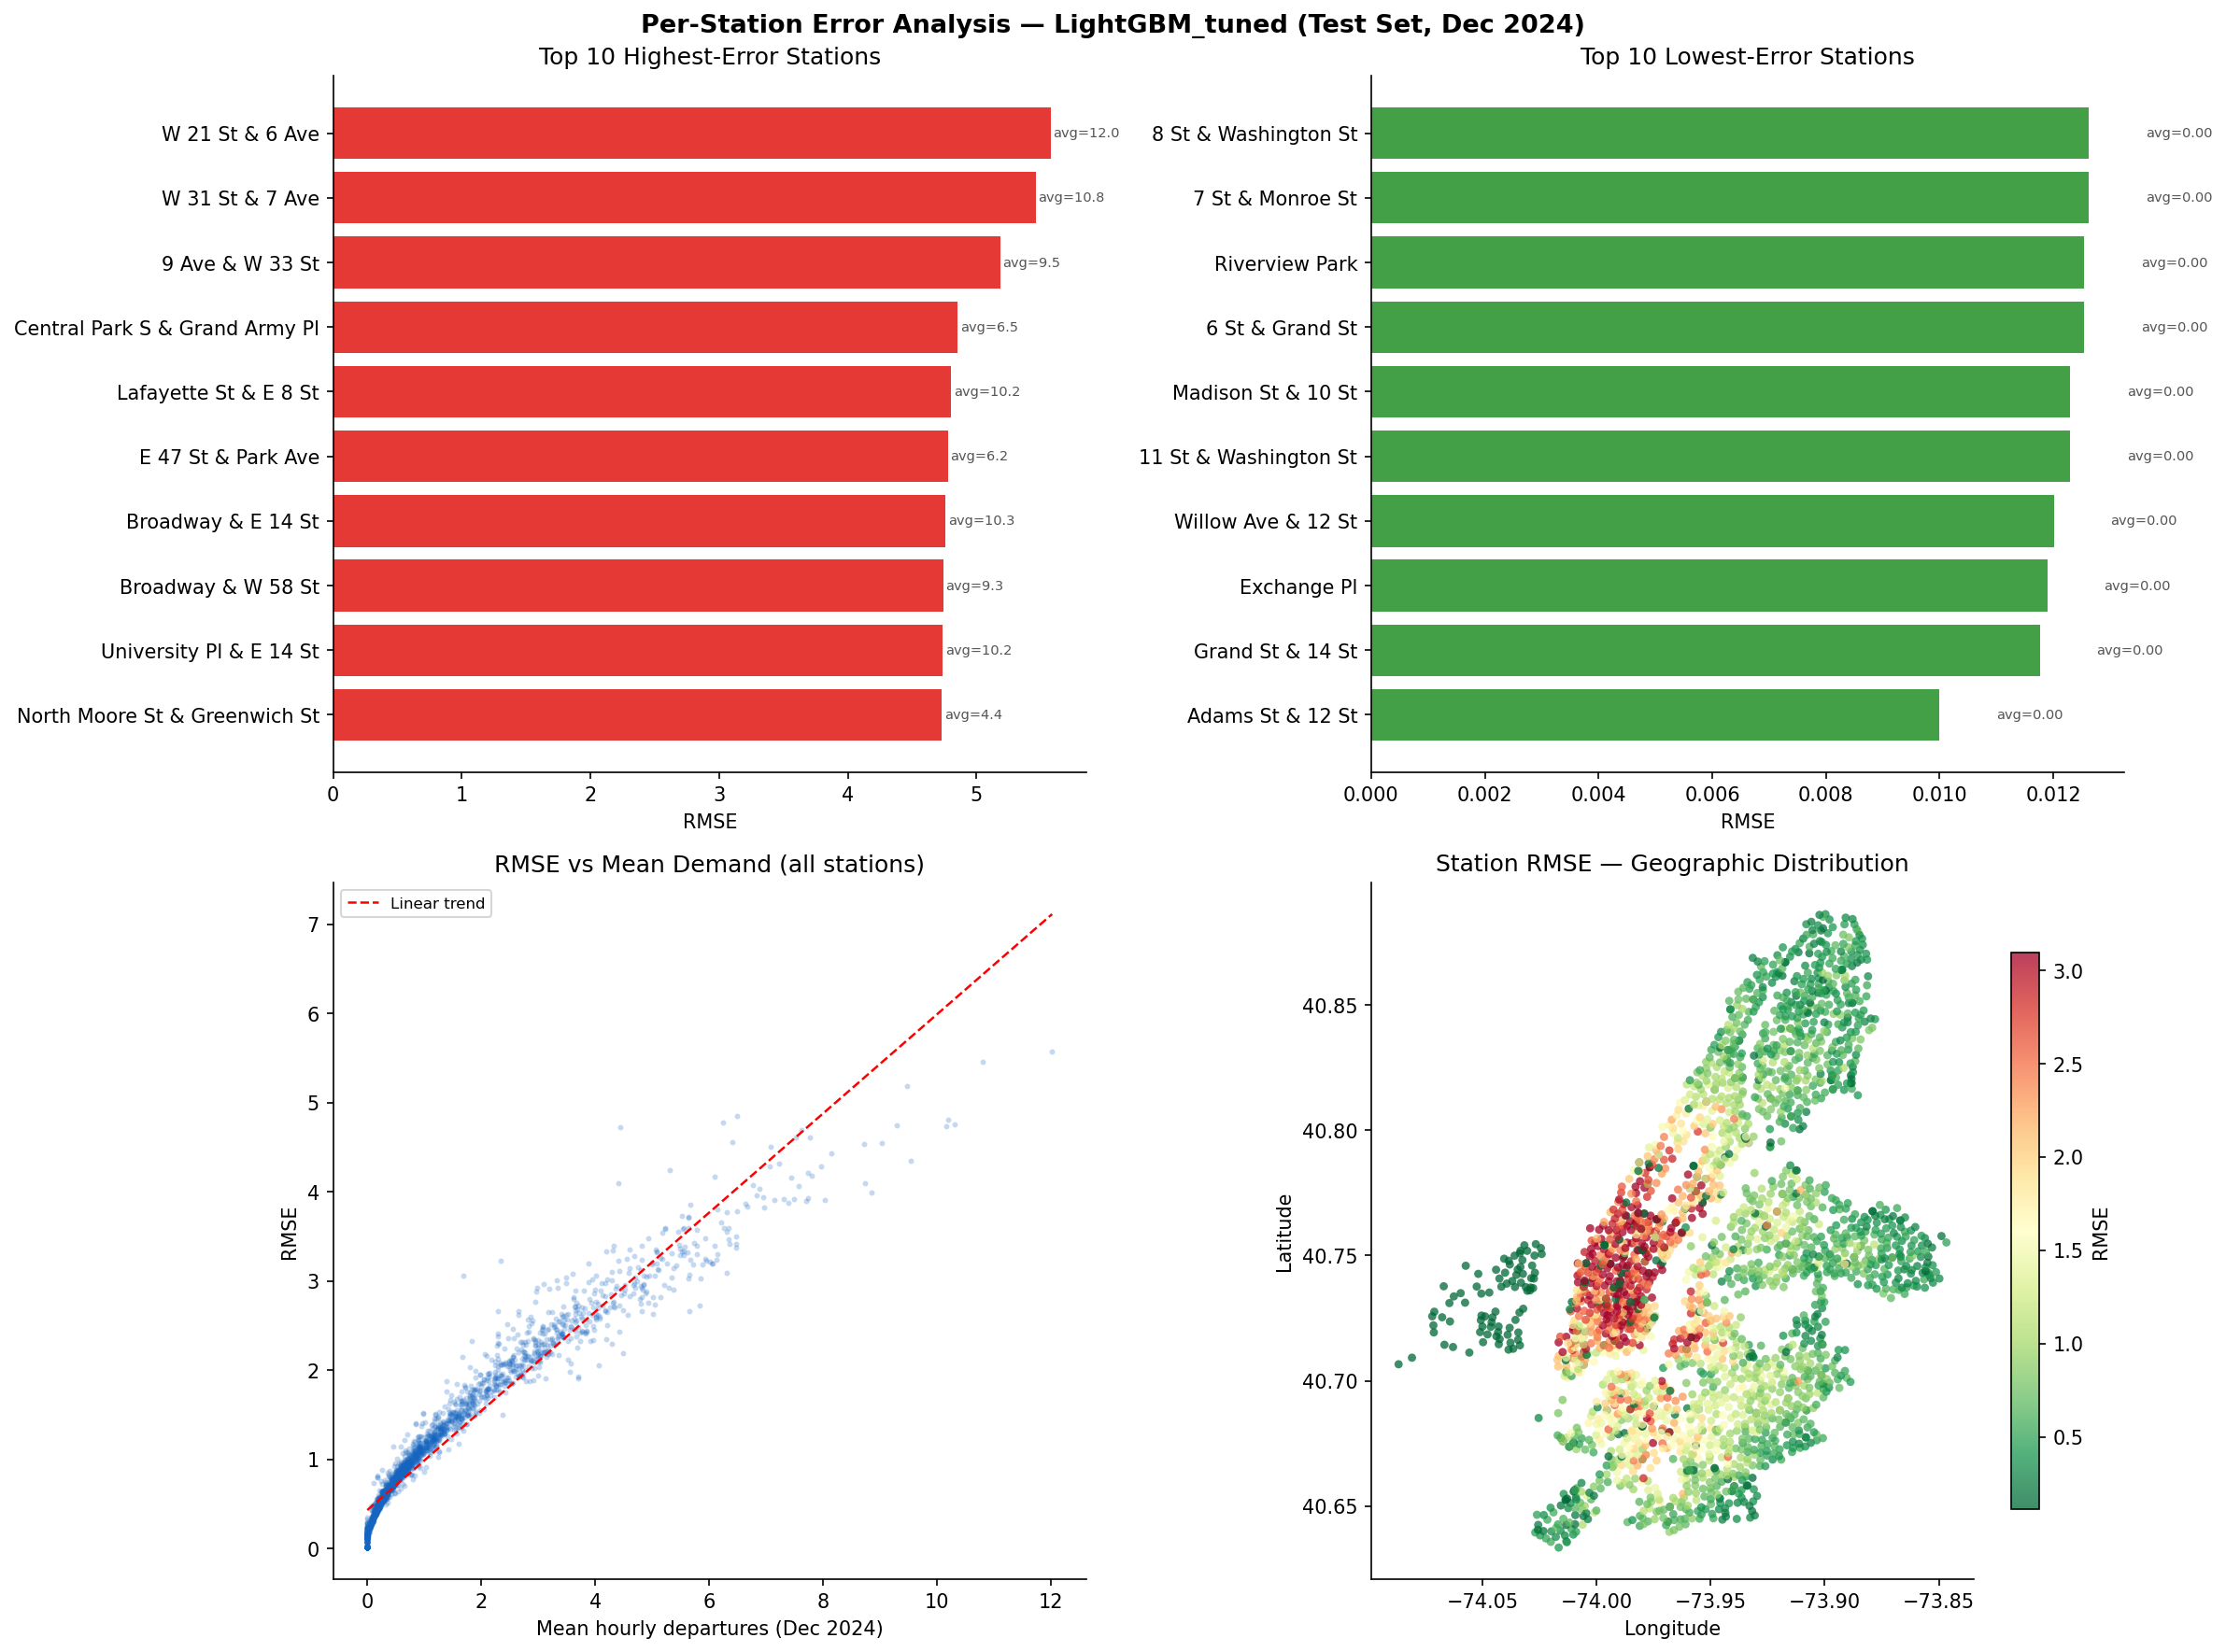
\includegraphics[width=0.85\linewidth]{../results/station_error.png}
  \caption{Per-station RMSE on the test set. Left: geographic distribution.
           Right: RMSE vs.\ mean hourly demand.}
  \label{fig:station}
\end{figure}

Figure~\ref{fig:station} shows that errors concentrate in high-demand Midtown
and Lower Manhattan stations. The five highest-error stations (e.g.,
W~21~St~\&~6~Ave with RMSE = 5.58, W~31~St~\&~7~Ave with RMSE = 5.46) are all
in Manhattan and average 6--12 departures per hour. In contrast, outer-borough
stations with near-zero demand are trivially easy to predict. The right panel
confirms a strong positive relationship between mean demand and RMSE, consistent
with the patterns seen in the error distribution analysis.

This geographic concentration of errors is consistent with
\citet{cortez2023scalability}, who also find that large, high-demand systems
like NYC Citi Bike are harder to forecast than smaller systems.

\subsection{Actual vs.\ Predicted}

\begin{figure}[H]
  \centering
  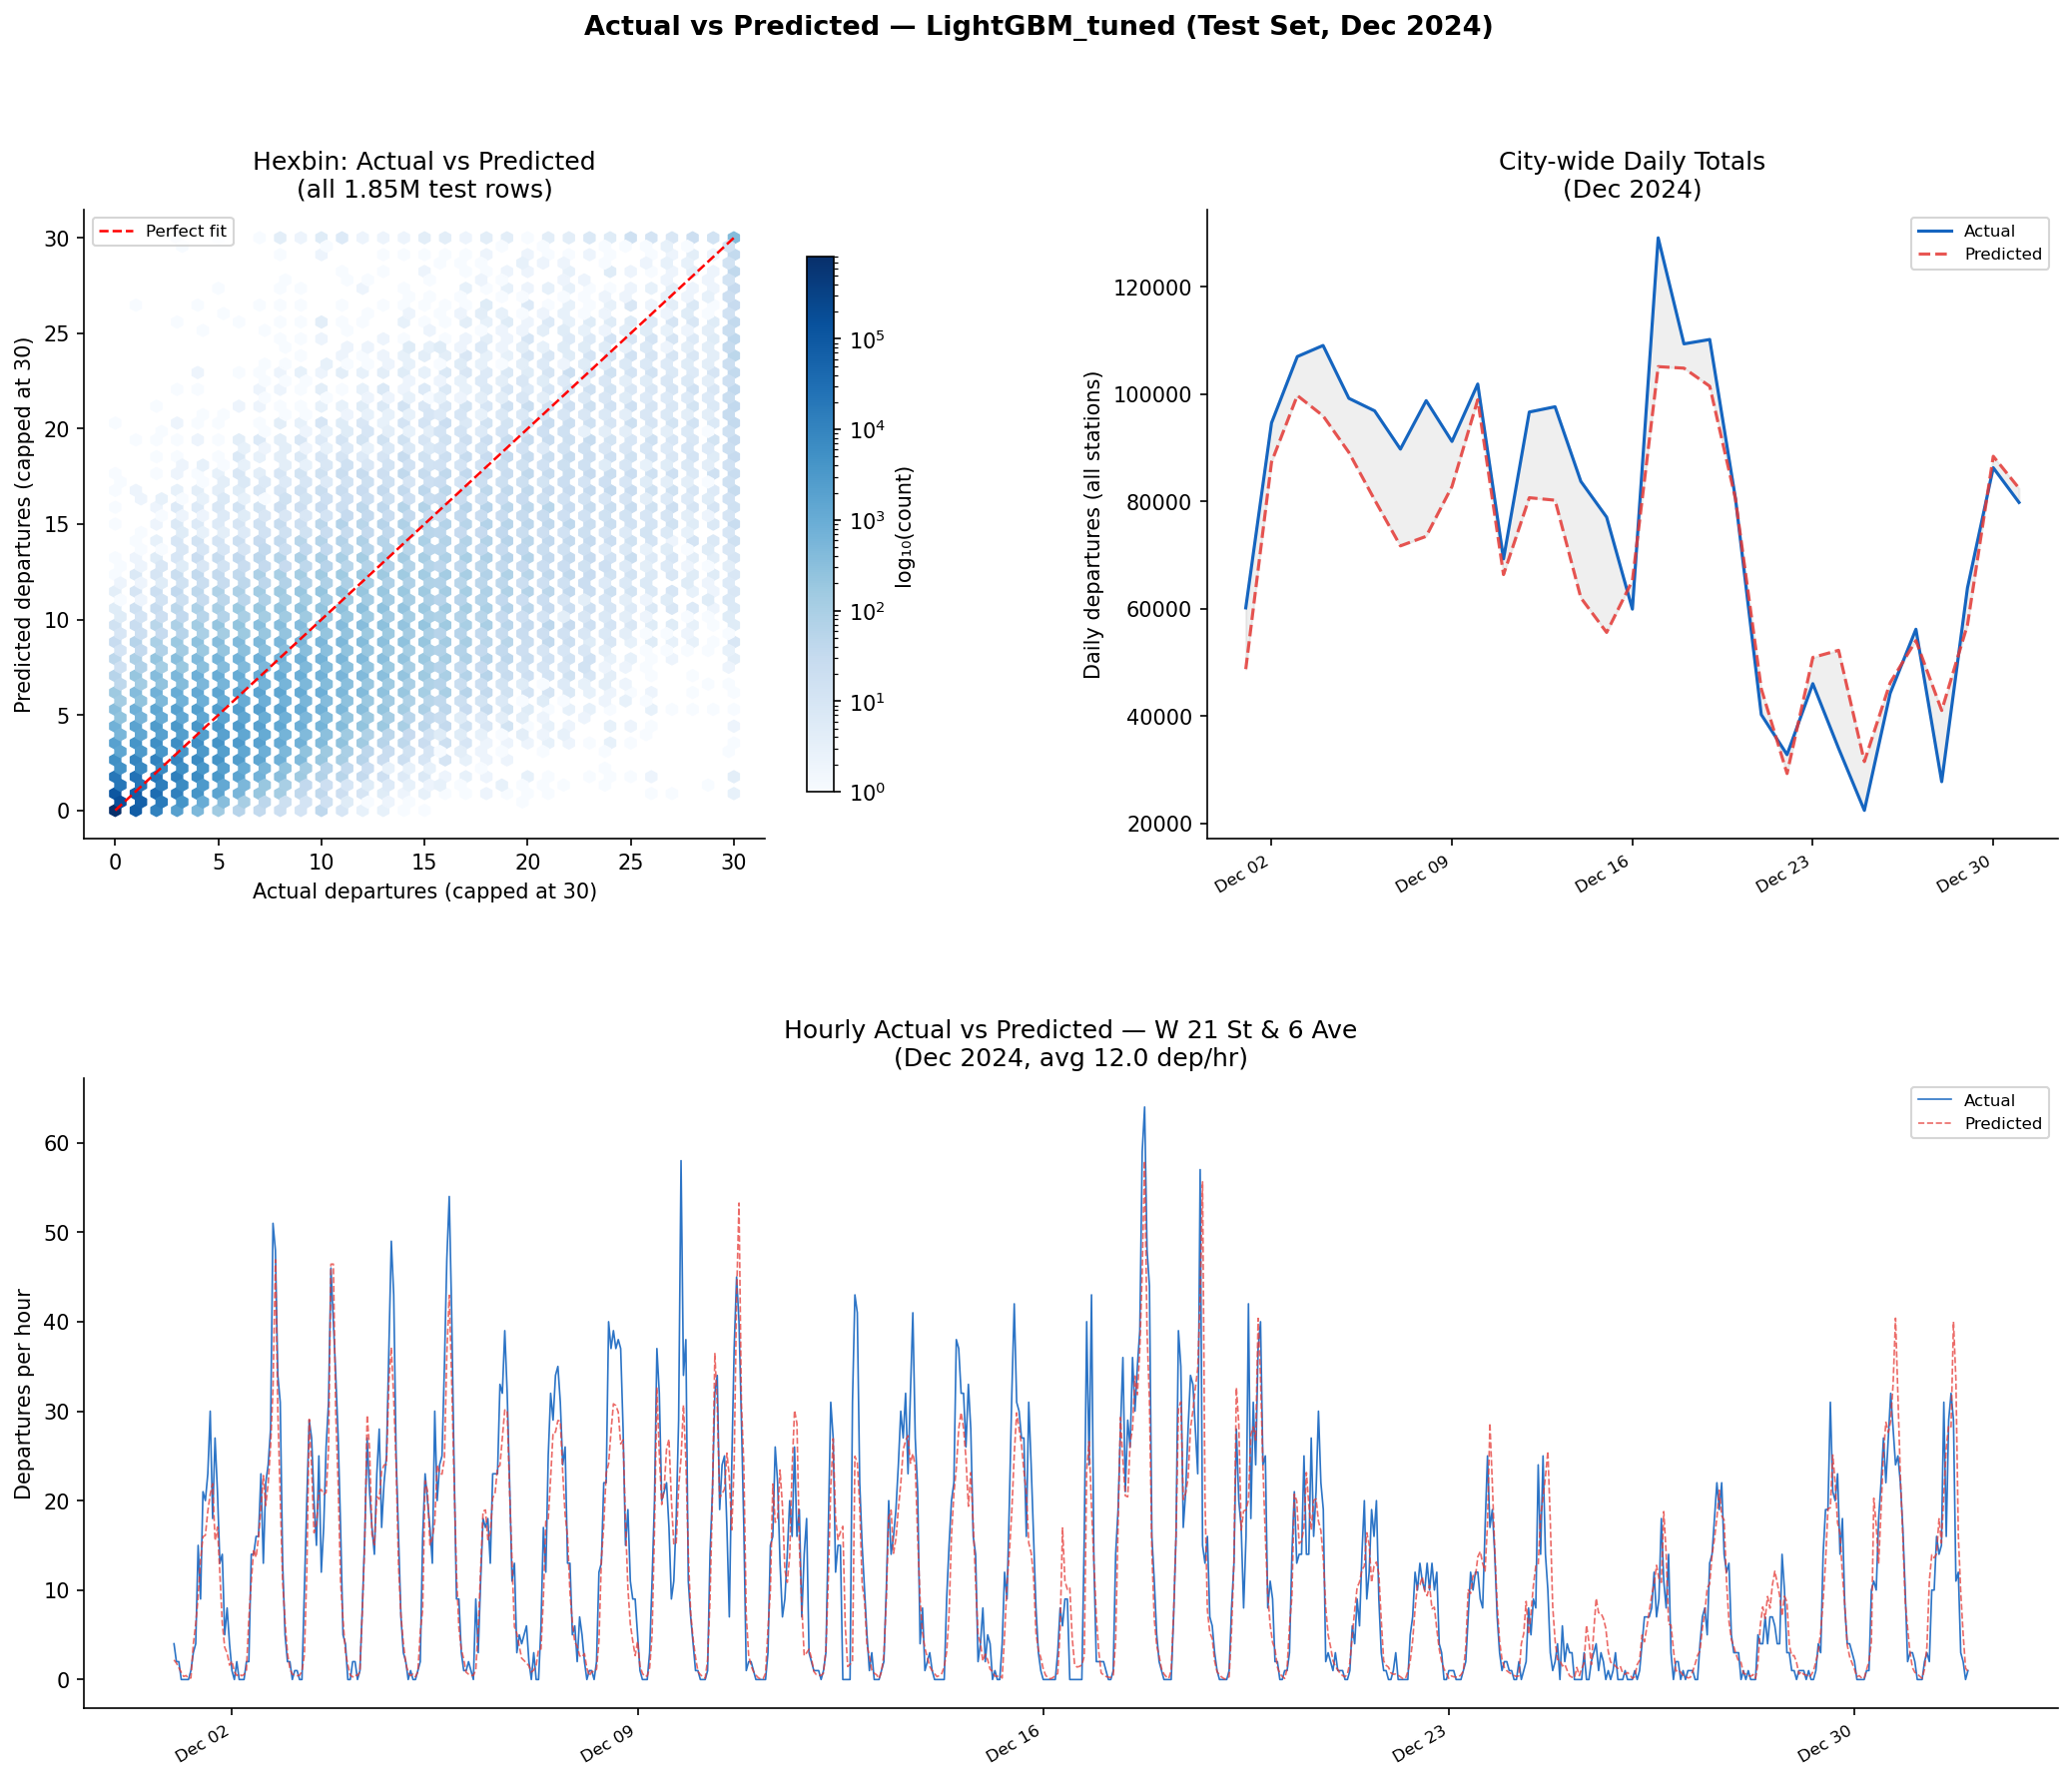
\includegraphics[width=0.85\linewidth]{../results/actual_vs_pred.png}
  \caption{Actual vs.\ predicted departures. Left: hexbin scatter on test set.
           Center: city-wide daily totals. Right: single high-demand station.}
  \label{fig:avp}
\end{figure}

Figure~\ref{fig:avp} provides three complementary views of model fit. The
hexbin scatter shows that predictions are tightly concentrated along the
diagonal for low-demand hours, with increasing spread at higher values. The
city-wide daily totals track closely with actual ridership across December,
including the Christmas holiday dip (December 24--26). At the busiest station
(W~21~St~\&~6~Ave, RMSE = 5.58), the model captures the daily demand cycle
well but systematically underestimates the largest peaks.

\subsection{Sample Complexity}

\begin{figure}[H]
  \centering
  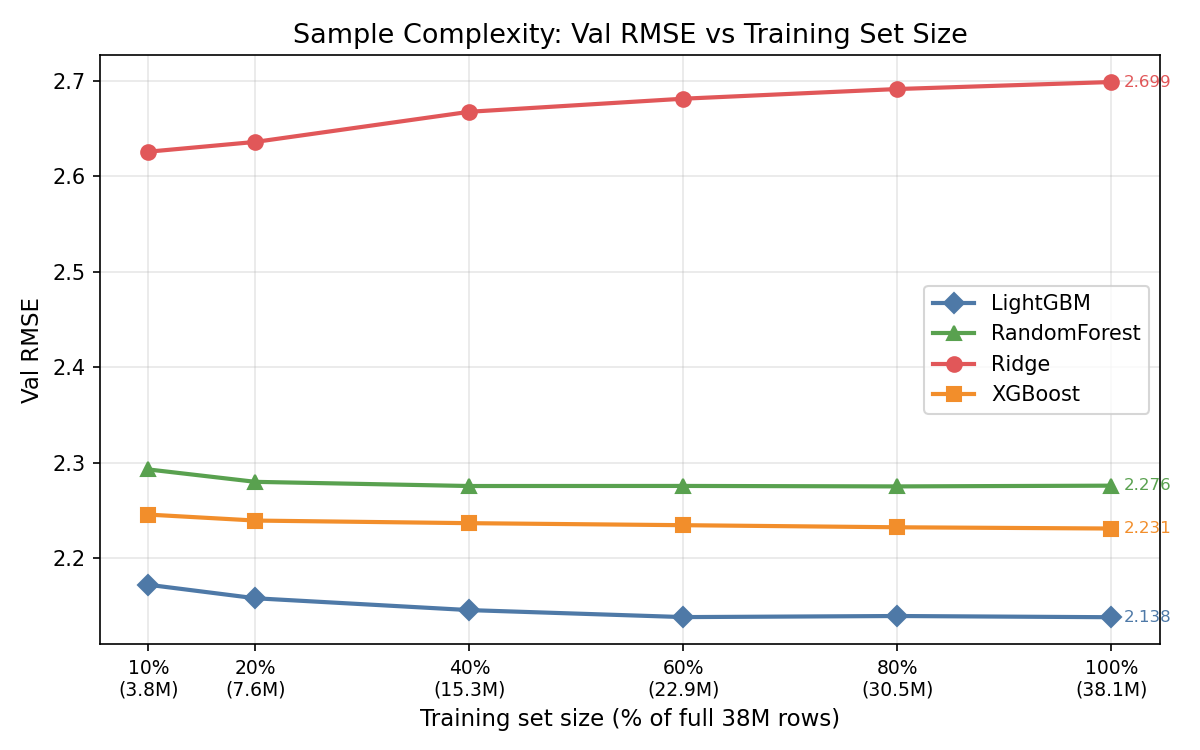
\includegraphics[width=0.75\linewidth]{../results/sample_complexity.png}
  \caption{Validation RMSE as a function of training set size for Ridge,
           XGBoost, LightGBM, and Random Forest. Random Forest is capped at
           10M rows due to scaling constraints.}
  \label{fig:sample}
\end{figure}

To understand how each model's performance scales with data, we trained
Ridge, XGBoost, LightGBM, and Random Forest on six fractions of the training
set: 10\%, 20\%, 40\%, 60\%, 80\%, and 100\% (corresponding to roughly
3.8M to 38.1M rows). The validation set is fixed at Oct--Nov 2024 across all
runs. Table~\ref{tab:sample} reports validation RMSE at each fraction.

\begin{table}[H]
\centering
\caption{Validation RMSE vs.\ training set size.}
\label{tab:sample}
\begin{tabular}{lcccccc}
\toprule
Frac & 10\% & 20\% & 40\% & 60\% & 80\% & 100\% \\
Train rows & 3.8M & 7.6M & 15.3M & 22.9M & 30.5M & 38.1M \\
\midrule
Ridge        & 2.626 & 2.636 & 2.667 & 2.681 & 2.691 & 2.699 \\
XGBoost      & 2.245 & 2.239 & 2.237 & 2.234 & 2.232 & 2.231 \\
LightGBM     & 2.172 & 2.158 & 2.145 & 2.138 & 2.139 & 2.138 \\
Random Forest & 2.293 & 2.280 & 2.275 & 2.275 & 2.276 & 2.276 \\
\bottomrule
\end{tabular}
\end{table}

Three patterns emerge from Figure~\ref{fig:sample}. First, LightGBM's
validation RMSE drops by only 0.034 as the training set grows tenfold,
and the curve is essentially flat from 40\% onward. This indicates that
3.8M rows already capture most of the learnable signal --- the remaining
34M rows yield diminishing returns. Second, Ridge Regression actually
\emph{degrades} slightly with more data (2.626 $\rightarrow$ 2.699). Because
the regularization strength $\alpha=1$ is fixed, its relative effect weakens
as the dataset grows; combined with the mild seasonal distribution shift
between training (Jan 2023 -- Sep 2024) and validation (Oct -- Nov 2024),
this leads to slightly worse generalization. Third, the model ranking
LightGBM $>$ XGBoost $>$ Random Forest $>$ Ridge is stable across all
fractions; additional data shrinks the gaps between models but never
changes the ordering.

The most important takeaway is that the bottleneck on this task is
\textbf{feature expressiveness, not data quantity}. All nonlinear models
saturate well before the full training set is consumed. Future improvements
are more likely to come from richer features --- weather lag/lead variables,
station embeddings, or cluster-level aggregates --- than from collecting
more data.

% ── 7. Conclusion ─────────────────────────────────────────────────────────────
\section{Conclusion}

We developed a machine learning pipeline to predict hourly bike departure counts
across NYC Citi Bike stations. The tuned LightGBM model achieves test RMSE =
1.501 and MAE = 0.759 across 1.85 million station-hour observations in December
2024, outperforming both simpler baselines and prior deep learning approaches on
the same dataset.

Our analysis reveals several consistent patterns. Short-term lag features
dominate: the three lag variables account for 85\% of feature importance gain,
confirming that recent demand history is far more informative than weather or
calendar features alone. Errors scale with demand level, with the PM rush hour
and high-demand Midtown Manhattan stations being the hardest cases. Day of week
has little impact, while colder months with lower peak demand are easier to
predict.

Possible directions for future work include station-level embeddings or
clustering to better capture neighborhood-specific demand patterns, separate
models for high-demand and low-demand stations, weather features modeled as a
time series rather than a fixed snapshot, and prediction of arrivals alongside
departures to support rebalancing decisions.

% ── References ────────────────────────────────────────────────────────────────
\bibliographystyle{plainnat}
\bibliography{references}

\end{document}
